%%%%%%%%%%%%%%%%%%%%%%%%%%%%%%%%%%%%%%%%%%%%%%%%%%%%%%%%%%%%%%%%
%%                                                            %%
%%   essentialsOfLatin, Italian translation 2017              %%
%%                                                            %%
%% From:  Henry C. Pearson, Essentials Of Latin For Beginners %%
%%        (1915, New York, American Book Company)             %%
%%                                                            %%
%%    https://archive.org/details/essentialslatin04peargoog   %%
%%                                                            %%
%% Translated by g.p.ciceri <gp.ciceri@gmail.com>             %%
%% ---------------------------------------------------------- %%
%% This translation is Licensed under                         %%
%% Creative Commons Attribution-ShareAlike 4.0 International  %%
%% https://creativecommons.org/licenses/by-sa/4.0/            %%
%%                                                            %%
%%%%%%%%%%%%%%%%%%%%%%%%%%%%%%%%%%%%%%%%%%%%%%%%%%%%%%%%%%%%%%%%

% āēīōū
% ăĕĭŏŭ




\documentclass[nols]{tufte-handout}

%\geometry{showframe} % display margins for debugging page layout

\usepackage{fontspec}
\usepackage{ifxetex}
\setmainfont[Path=./fonts/palatino-linotype/, ItalicFont=palai.ttf, BoldFont=palab.ttf]{pala.ttf}


% \defaultfontfeatures{Mapping=tex-text}
% \setromanfont[Path=./fonts/TeX-Gyre-Schola/,Mapping=tex-text]{TeX Gyre Schola}
% \setsansfont[Path=./fonts/TeX-Gyre-Heros/,Scale=MatchLowercase,Mapping=tex-text]{TeX Gyre Heros}
% \setmonofont[Path=./fonts/TeX-Gyre-Cursor/,Scale=MatchLowercase]{TeX Gyre Cursor}

\usepackage{lipsum}
\usepackage{url}
\usepackage{longtable}
\usepackage{stackengine}

\usepackage{graphicx} % allow embedded images
  \setkeys{Gin}{width=\linewidth,totalheight=\textheight,keepaspectratio}
  \graphicspath{{graphics/}} % set of paths to search for images
\usepackage{amsmath}  % extended mathematics
\usepackage{booktabs} % book-quality tables
\usepackage{units}    % non-stacked fractions and better unit spacing
\usepackage{multicol} % multiple column layout facilities
\usepackage{lipsum}   % filler text
\usepackage{fancyvrb} % extended verbatim environments
  \fvset{fontsize=\normalsize}% default font size for fancy-verbatim environments

% Standardize command font styles and environments
\newcommand{\doccmd}[1]{\texttt{\textbackslash#1}}% command name -- adds backslash automatically
\newcommand{\docopt}[1]{\ensuremath{\langle}\textrm{\textit{#1}}\ensuremath{\rangle}}% optional command argument
\newcommand{\docarg}[1]{\textrm{\textit{#1}}}% (required) command argument
\newcommand{\docenv}[1]{\textsf{#1}}% environment name
\newcommand{\docpkg}[1]{\texttt{#1}}% package name
\newcommand{\doccls}[1]{\texttt{#1}}% document class name
\newcommand{\docclsopt}[1]{\texttt{#1}}% document class option name
\newenvironment{docspec}{\begin{quote}\noindent}{\end{quote}}% command specification environment

% concetti morfosintattici
\usepackage{xspace} 
\newcommand{\noun}{\textsc{sostantivo}\xspace}
\newcommand{\nouns}{\textsc{sostantivi}\xspace}
\newcommand{\adject}{\textsc{aggettivo}\xspace}
\newcommand{\adjects}{\textsc{aggettivi}\xspace}
\newcommand{\gnumber}{\textsc{numero}\xspace}
\newcommand{\gnumbers}{\textsc{numeri}\xspace}
\newcommand{\gender}{\textsc{genere}\xspace}
\newcommand{\genders}{\textsc{generi}\xspace}
\newcommand{\gcase}{\textsc{caso}\xspace}
\newcommand{\gcases}{\textsc{casi}\xspace}
\newcommand{\tense}{\textsc{tempo}\xspace}
\newcommand{\mood}{\textsc{modo}\xspace}
\newcommand{\gverb}{\textsc{verbo}\xspace}
\newcommand{\gverbs}{\textsc{verbi}\xspace}
\newcommand{\adjective}{\textsc{aggettivo}\xspace}
\newcommand{\nom}{\textsc{nom}\xspace}
\newcommand{\gen}{\textsc{gen}\xspace}
\newcommand{\dat}{\textsc{dat}\xspace}
\newcommand{\acc}{\textsc{acc}\xspace}
\newcommand{\voc}{\textsc{voc}\xspace}
\newcommand{\abl}{\textsc{abl}\xspace}
\newcommand{\gexit}{\textsc{uscita}\xspace}
\newcommand{\gexits}{\textsc{uscite}\xspace}
\newcommand{\declinazione}{\textsc{declinazione}\xspace}
\newcommand{\masc}{\textsc{maschile}\xspace}
\newcommand{\femm}{\textsc{femminile}\xspace}
\newcommand{\neut}{\textsc{neutro}\xspace}

\newcommand{\indic}{\textsc{indicativo}\xspace}
\newcommand{\imper}{\textsc{imperativo}\xspace}
\newcommand{\gcong}{\textsc{congiuntivo}\xspace}
\newcommand{\ott}{\textsc{ottativo}\xspace}
\newcommand{\partic}{\textsc{participio}\xspace}
\newcommand{\infin}{\textsc{infinito}\xspace}

\newcommand{\pres}{\textsc{presente}\xspace}
\newcommand{\imperf}{\textsc{imperfetto}\xspace}
\newcommand{\aor}{\textsc{aoristo}\xspace}
\newcommand{\fut}{\textsc{futuro}\xspace}
\newcommand{\perf}{\textsc{perfetto}\xspace}
\newcommand{\pperf}{\textsc{piuccheperfetto}\xspace}

\newcommand{\sing}{\textsc{singolare}\xspace}
\newcommand{\plur}{\textsc{plurale}\xspace}
\newcommand{\dual}{\textsc{duale}\xspace}

\newcommand{\si}{\textsc{sing}\xspace}
\newcommand{\pl}{\textsc{plur}\xspace}
\newcommand{\du}{\textsc{dual}\xspace}

\newcommand{\att}{\textsc{attivo}\xspace}
\newcommand{\med}{\textsc{medio}\xspace}
\newcommand{\pass}{\textsc{passivo}\xspace}
\newcommand{\medpass}{\textsc{medio-passivo}\xspace}


% italianitudini
\renewcommand{\figurename}{Figura}
\renewcommand{\tablename}{Tabella}
\renewcommand{\contentsname}{Indice}

% fix per un qualche problema
\ifxetex
  \newcommand{\textls}[2][5]{%
    \begingroup\addfontfeatures{LetterSpace=#1}#2\endgroup
  }
  \renewcommand{\allcapsspacing}[1]{\textls[15]{#1}}
  \renewcommand{\smallcapsspacing}[1]{\textls[10]{#1}}
  \renewcommand{\allcaps}[1]{\textls[15]{\MakeTextUppercase{#1}}}
  \renewcommand{\smallcaps}[1]{\smallcapsspacing{\scshape\MakeTextLowercase{#1}}}
  \renewcommand{\textsc}[1]{\smallcapsspacing{\textsmallcaps{#1}}}
\fi

% too many float...
\extrafloats{100}

\title{Essentials Of Latin. Elementi di Latino. \newline Lezione XXII - Perfetto, Piuccheperfetto e Futuro Perfetto Passivo per la I e II coniugazione.}

\author[gpciceri]{a cura di Milagathòs: Milo's help to enjoy humanities.}

\date{21 Febbrajo 2017} % without \date command, current date is supplied


\begin{document}

\hyphenation{co-niu-ga-zio-ne}

\maketitle% this prints the handout title, author, and date

\begin{marginfigure}[-2.5cm]
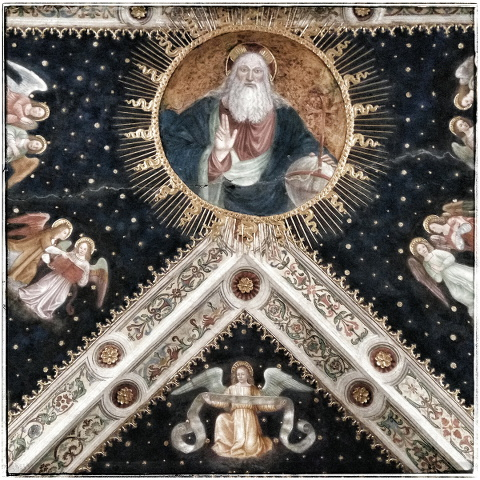
\includegraphics{smallthumb-lesson_XI.jpeg}
\setfloatalignment{b}
\end{marginfigure}


\begin{abstract}
\noindent
Queste lezioni riprendono il testo introduttivo al Latino di Pearson\cite{pearson1915}, del quale seguono la numerazione; la struttura di ogni lezione è piuttosto regolare: inizia con \textsc{cenni di morfologia e di sintassi latina}, seguita da un \textsc{piccolo vocabolario} per il lessico; ci sono infine vari \textsc{esercizi} di traduzione e di composizione latina.

\bigskip
\noindent
Lezione XXI - Perfetto, Piuccheperfetto e Futuro Perfetto Indicativo Passivo per la I e II coniugazione. Vocabolario, esercizi.
\end{abstract}

%\printclassoptions

\newthought{152.} Ripassa i punti 39., 81. e 86. Il perfetto, il piuccheperfetto e il futuro perfetto di tutti i verbi latini presentano forma composta, costruita con il participio perfetto (passivo) e, rispettivamente, con i tempi presente, imperfetto e futuro del verbo ausiliare essere \textbf{sum}. Il participio si comporta come un aggettivo al nominativo, concorda quindi con il soggetto del verbo anche in genere e numero. 

\begin{fullwidth}
\begin{table}[!htbp]
  \centering
  \begin{tabular}{l l l l l l}
    %\toprule
	& \multicolumn{5}{c}{\textsc{I Coniugazione - Perfetto Passivo di} \textbf{amō}} \\
	& \multicolumn{2}{c}{\textsc{Singolare}} & \hspace{10mm} & \multicolumn{2}{c}{\textsc{Plurale}} \\

    \textsc{1.} & amāt\textbf{us, a, um sum}, & \textit{io sono stato amato} & \hspace{10mm} & amāt\textbf{i, ae, a sumus}, & \textit{noi siamo stati amati} \\
    \textsc{2.} & amāt\textbf{us, a, um es}, & \textit{tu sei stato amato}   & \hspace{10mm} & amāt\textbf{i, ae, a estis}, & \textit{voi siete stati amati} \\
    \textsc{3.} & amāt\textbf{us, a, um est}, & \textit{egli è stato amato}  & \hspace{10mm} & amāt\textbf{i, ae, a sunt}, & \textit{essi sono stati amati} \\
	
	& \multicolumn{5}{c}{\textsc{Piuccheperfetto Passivo}} \\
	& \multicolumn{2}{c}{\textsc{Singolare}} & \hspace{10mm} & \multicolumn{2}{c}{\textsc{Plurale}} \\

    \textsc{1.} & amāt\textbf{us, a, um eram}, & \textit{io ero stato amato} & \hspace{10mm} & amāt\textbf{i, ae, a eramus}, & \textit{noi eravamo stati amati} \\
    \textsc{2.} & amāt\textbf{us, a, um eras}, & \textit{tu eri stato amato}   & \hspace{10mm} & amāt\textbf{i, ae, a eratis}, & \textit{voi eravate stati amati} \\
    \textsc{3.} & amāt\textbf{us, a, um erat}, & \textit{egli era stato amato}  & \hspace{10mm} & amāt\textbf{i, ae, a erant}, & \textit{essi erano stati amati} \\
	
	& \multicolumn{5}{c}{\textsc{Futuro Perfetto Passivo}} \\
	& \multicolumn{2}{c}{\textsc{Singolare}} & \hspace{10mm} & \multicolumn{2}{c}{\textsc{Plurale}} \\

    \textsc{1.} & amāt\textbf{us, a, um ero}, & \textit{io sarò stato amato} & \hspace{10mm} & amāt\textbf{i, ae, a erimus}, & \textit{noi saremo stati amati} \\
    \textsc{2.} & amāt\textbf{us, a, um eris}, & \textit{tu sarai stato amato}   & \hspace{10mm} & amāt\textbf{i, ae, a eritis}, & \textit{voi sarete stati amati} \\
    \textsc{3.} & amāt\textbf{us, a, um erit}, & \textit{egli sarà stato amato}  & \hspace{10mm} & amāt\textbf{i, ae, a erunt}, & \textit{essi saranno stati amati} \\

    %\bottomrule
  \end{tabular}
  %\caption{}
  \label{tab:normaltab}
  %\zsavepos{pos:normaltab}
\end{table}
\end{fullwidth}


\newthought{Osservazioni}
\begin{itemize}
\item[\textsc{1.}] Allo stesso modo, coniuga e poi traduci questi tempi per i verbi \textbf{moneō, videō, portō}.  
\item[\textsc{2.}] Osserva con cura che il participio è declinato come l'aggettivo della prima classe \textbf{bonus, a, um}, e che concorda con il soggetto; ad esempio:
	\begin{itemize}
	\item{\textit{Io (una ragazza) sono stata amata}} \textbf{amata sum}
	\item{\textit{Noi (ragazze) siamo state amate}} \textbf{amatae sumus}
	\item{\textit{la città era stata vista}} \textbf{oppidum visum erat}
	\item{\textit{la ragazza è stata amata}} \textbf{puella amata est}
	\end{itemize}  
\item[\textsc{3.}] Per la differenza di significato tra il perfetto e l'imperfetto passivo vedi il punto 92., 2.  
\end{itemize}

% āēīōū
% ăĕĭŏŭ



\newthought{153. Vocabolario}

\begin{multicols}{2}
    \noindent \hangindent=1em \textbf{amicitia, -ae}, f., \textit{amicizia, alleanza}.  \\
    \noindent \hangindent=1em \textbf{pax, pacis}, f., \textit{pace}.  \\
	\noindent \hangindent=1em \textbf{mensis, mensis}, m., \textit{mese}.  \\
	\noindent \hangindent=1em \textbf{iter, itineris}, n., \textit{marcia, strada, viaggio} (501).  \\
	\noindent \hangindent=1em \textbf{ex itinere}, \textit{lungo il cammino}.  \\
	\noindent \hangindent=1em \textbf{civis, civis}, m. e f., \textit{cittadino, cittadina}.  \\
	\noindent \hangindent=1em \textbf{civitas, -atis}, f., \textit{stato, cittadinanza}.  \\
	\noindent \hangindent=1em \textbf{confirmō, -as, -avi, -atum, -are}, \textit{rinforzare, stabilire}.  \\
    \noindent \hangindent=1em \textbf{contineō, -es, continui, contentum, continēre}, \textit{tenere assieme, trattenere, limitare}.  \\
    
\end{multicols}


\newthought{154. Esercizi}
\\
\textsc{I.} \quad
\textsc{1.}~Vulnerati eratis; videbamus; incitatae sunt. \quad
\textsc{2.}~Laudatne est? Laudati erant; culpatae erunt. \quad
\textsc{3.}~Pax cum multis civitatibus est confirmata. \quad
\textsc{4.}~Cives ob amicitiam laudavimus. \quad
\textsc{5.}~Galli montibus et fluminibus continebantur. \quad
\textsc{6.}~Multa oppida decem mensibus occupata erant. \quad
\textsc{7.}~Multum Helvetiorum urbs ex itinere est expugnata. \quad
\textsc{8.}~Multum frumentum ex agris in hiberna portatum erat. \quad
\textsc{9.}~Caesar milites in castris habebat. \quad
\textsc{10.}~Multi homines a Romanis erant necati. \quad
\textsc{11.}~Multos civis in Italia vidimus. \quad
\textsc{12.}~Urbs ab imperatore magno cum studio oppugnata est.
\\
\textsc{II.} \quad
\textsc{1.}~Era trattenuta; voi eravate stati incolpati. \quad
\textsc{2.}~Noi (ragazze) saremo state lodate; essi sono stati ammoniti. \quad
\textsc{3.}~Pace e amicizia sono state stabilite con i Galli. \quad
\textsc{4.}~I cittadini erano stati sollevati dai loro capi. \quad
\textsc{5.}~La ragazza fu portata con cura in città. \quad
\textsc{6.}~I soldati furono lodati dal generale per il loro coraggio. \quad
\textsc{7.}~Cesare attaccò una città degli Elvezi lungo il cammino. \quad
\textsc{8.}~La cavalleria era stata colpita dalle armi del nemico.

\begin{figure}[!b]
  %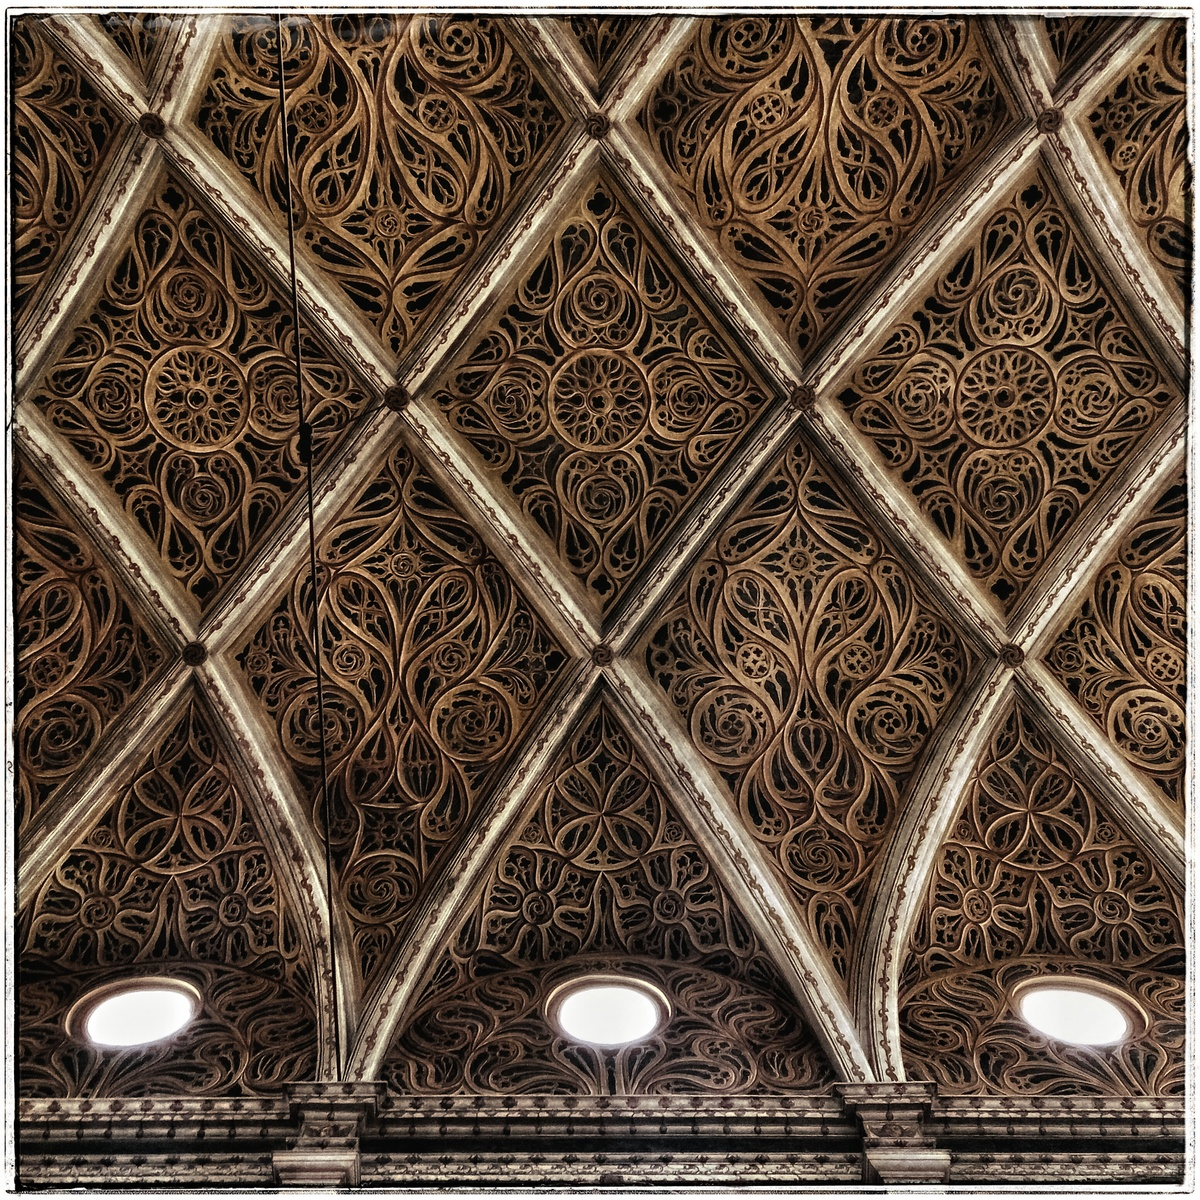
\includegraphics{thumb-lesson_XXI.jpeg}
  %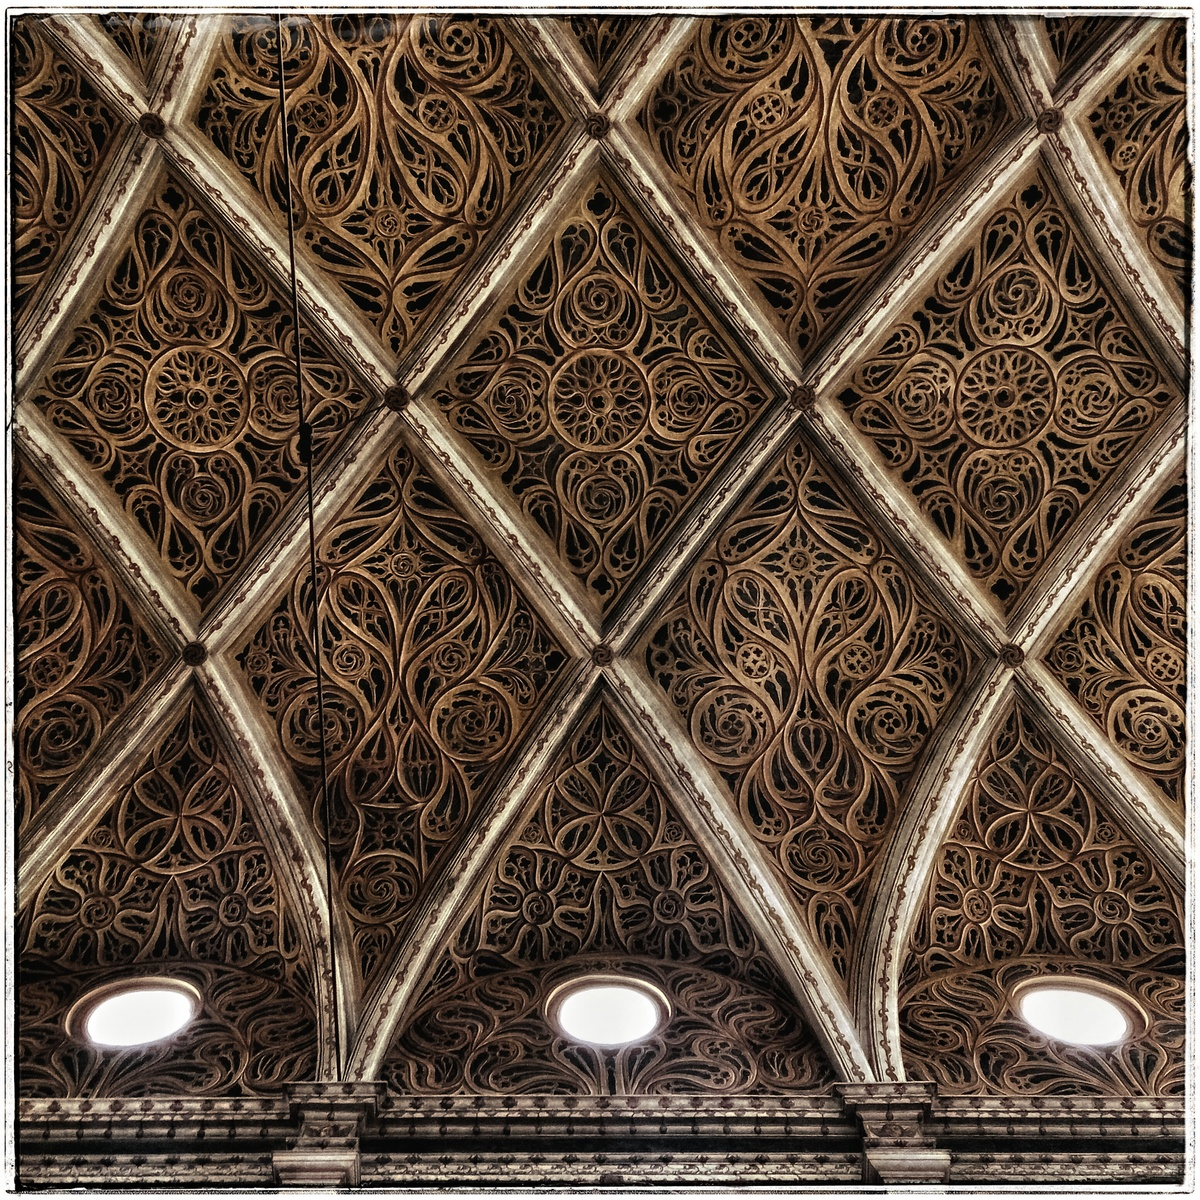
\includegraphics[width=0.9\linewidth]{thumb-lesson_XXI.jpeg}
  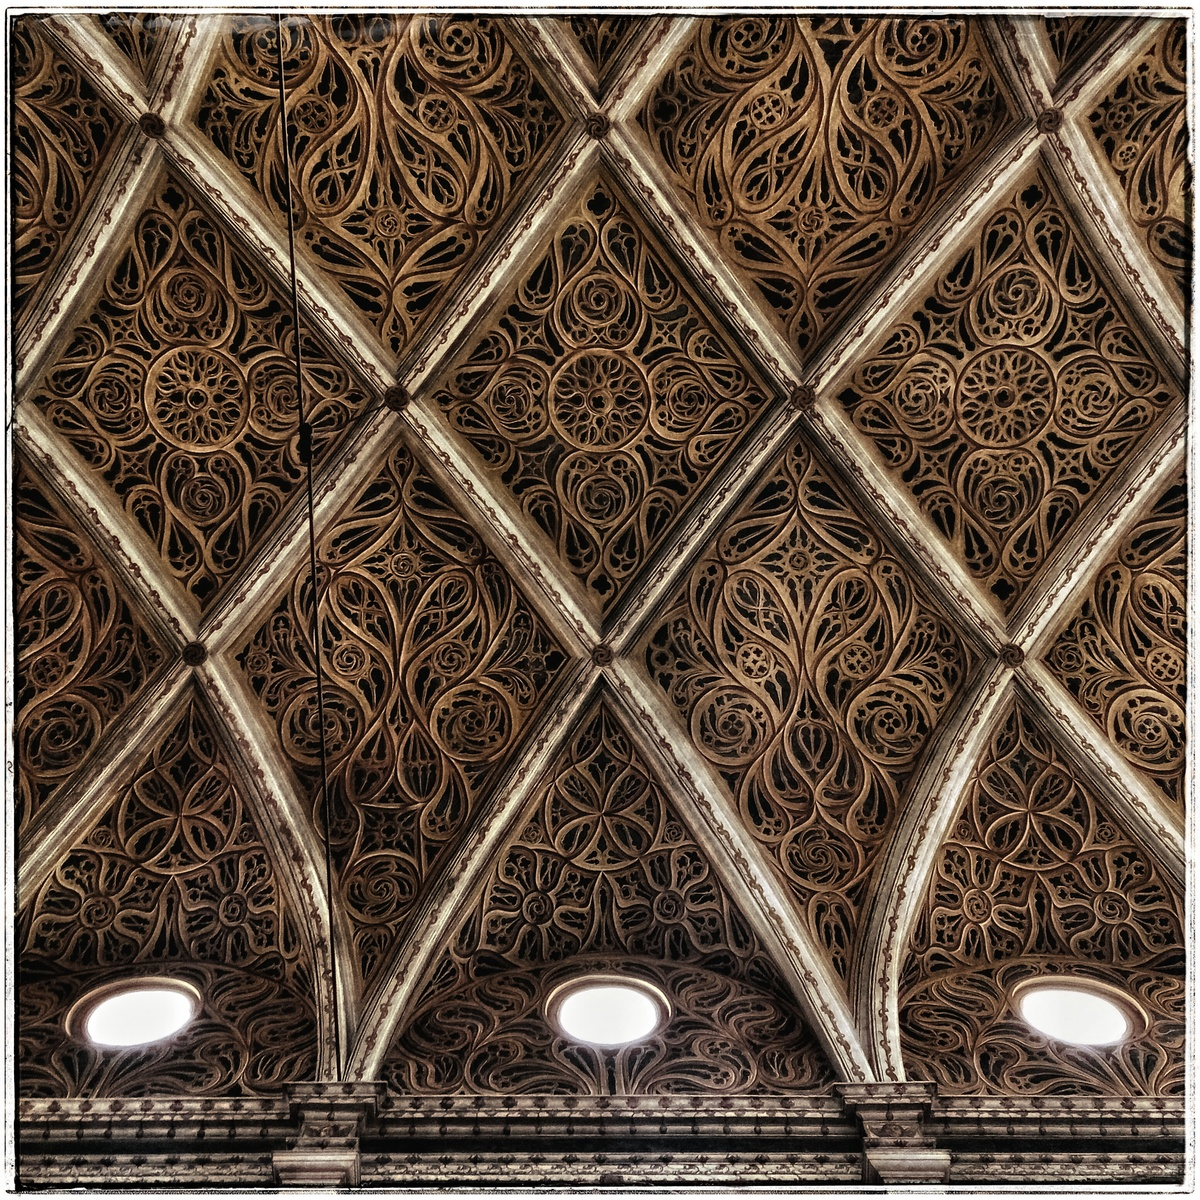
\includegraphics{thumb-lesson_XXI.jpeg}
  \caption{Milano: San Maurizio al Monastero Maggiore}
  \label{fig:textfig}
  %\zsavepos{pos:textfig}
  %\setfloatalignment{b}
\end{figure}

 

\nobibliography{latinBiblio}
\bibliographystyle{alpha}


\end{document}
